\documentclass{article}
\usepackage{graphicx}
\usepackage{geometry}
\usepackage{hyperref}
\usepackage{booktabs}
\usepackage{subcaption}
\usepackage{amsmath}

\geometry{
    a4paper,
    margin=0.7in
}

\hypersetup{
    colorlinks=true,
    linkcolor=blue,
    filecolor=magenta,      
    urlcolor=cyan,
}

\title{SNN Surrogate Gradient $\alpha$ Parameter Comparison\\Robustness Sweep under Data Heterogeneity ($f \le 3$)}
\author{ByzFL SNN Benchmark}
\date{\today}

\begin{document}

\maketitle

\section{Introduction}
This document presents a detailed comparison of the Spiking Neural Network (SNN) robustness on the MNIST dataset using different scaling factors $\alpha$ for the ArcTangent (\texttt{atan}) surrogate gradient. The evaluation spans:
\begin{itemize}
    \item \textbf{Surrogate Gradient Scaling}: $\alpha \in \{1.0, 1.25, 1.5, 2.0, 3.0\}$
    \item \textbf{Byzantine Nodes}: $f \in \{0, 1, 2, 3\}$ out of $N=10$ total nodes
    \item \textbf{Data Heterogeneity}: Non-IID levels $\gamma \in \{1.0, 0.66, 0.33, 0.0\}$ (where $\gamma = 0.0$ represents extreme Non-IID client partitions)
    \item \textbf{Attack Model}: Optimal A Little Is Enough (\texttt{Optimal\_ALittleIsEnough\_neg1})
    \item \textbf{Aggregators}: Best aggregated result across Centered Clipping and Geometric Median (pre-aggregated with NNM and ARC).
\end{itemize}

\section{Aggregated Test Accuracy Heatmaps}
The figure below displays the grid layout of the best aggregated test accuracy heatmaps for each tested $\alpha$ parameter value.

\begin{figure}[htbp]
    \centering
    \begin{subfigure}[b]{0.48\textwidth}
        \centering
        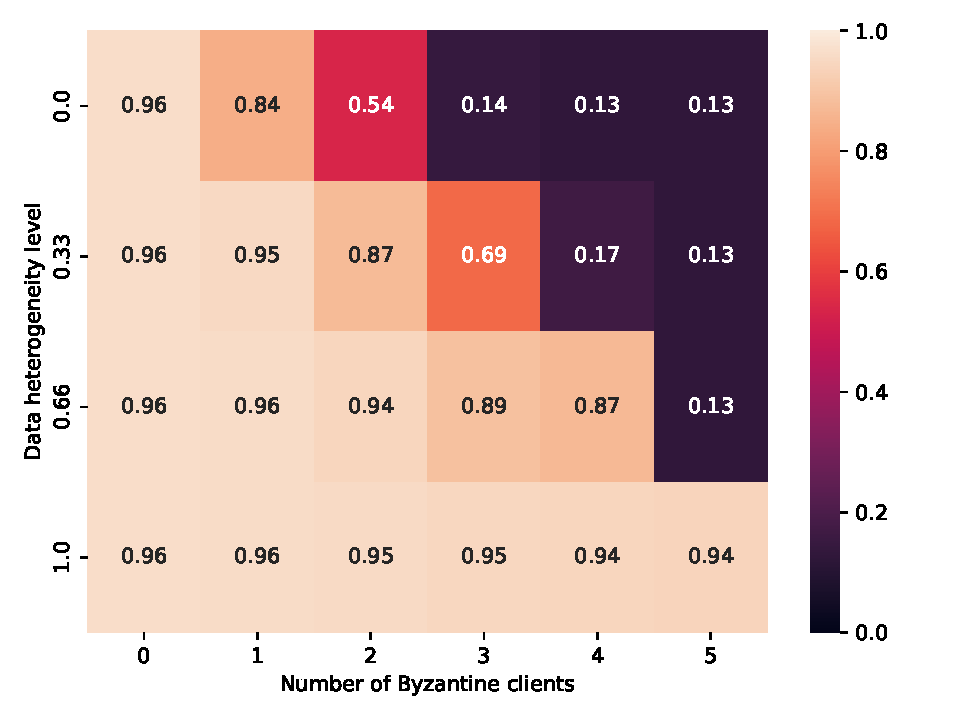
\includegraphics[width=\textwidth]{heatmap_alpha_1_0.pdf}
        \caption{$\alpha = 1.0$}
        \label{fig:alpha_1_0}
    \end{subfigure}
    \hfill
    \begin{subfigure}[b]{0.48\textwidth}
        \centering
        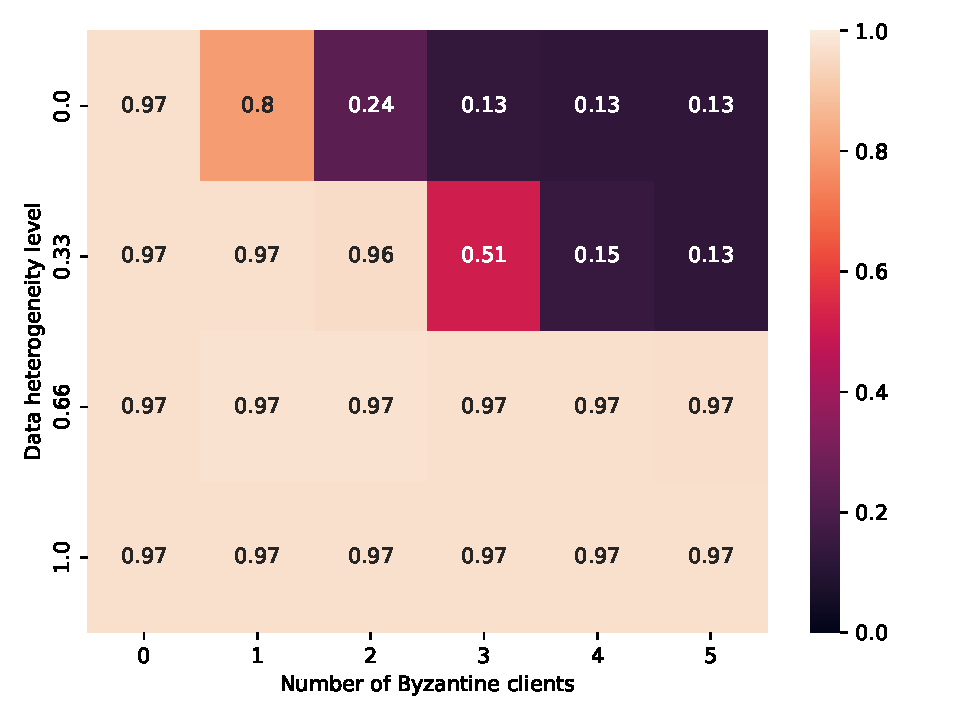
\includegraphics[width=\textwidth]{heatmap_alpha_1_25.pdf}
        \caption{$\alpha = 1.25$}
        \label{fig:alpha_1_25}
    \end{subfigure}
    
    \vspace{0.3cm}
    
    \begin{subfigure}[b]{0.48\textwidth}
        \centering
        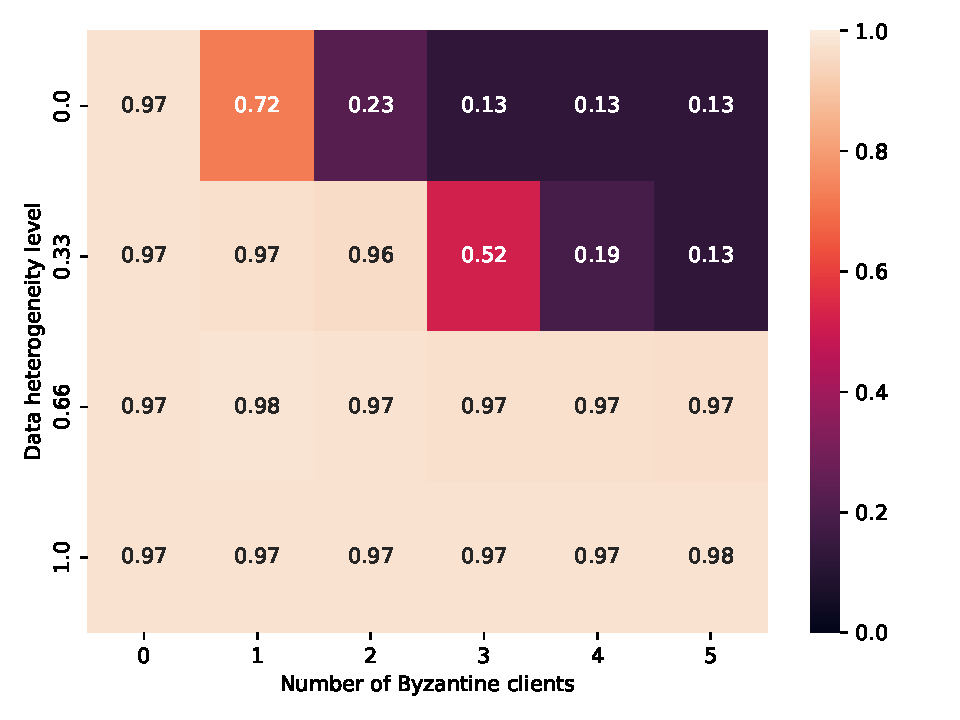
\includegraphics[width=\textwidth]{heatmap_alpha_1_5.pdf}
        \caption{$\alpha = 1.5$}
        \label{fig:alpha_1_5}
    \end{subfigure}
    \hfill
    \begin{subfigure}[b]{0.48\textwidth}
        \centering
        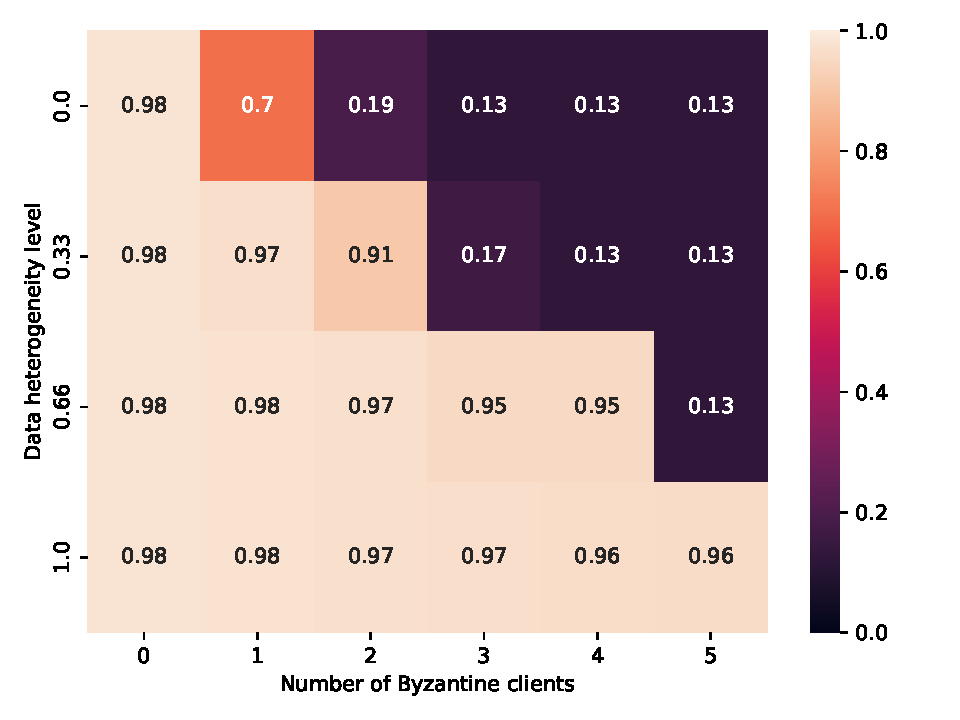
\includegraphics[width=\textwidth]{heatmap_alpha_2_0.pdf}
        \caption{$\alpha = 2.0$}
        \label{fig:alpha_2_0}
    \end{subfigure}
    
    \vspace{0.3cm}
    
    \begin{subfigure}[b]{0.48\textwidth}
        \centering
        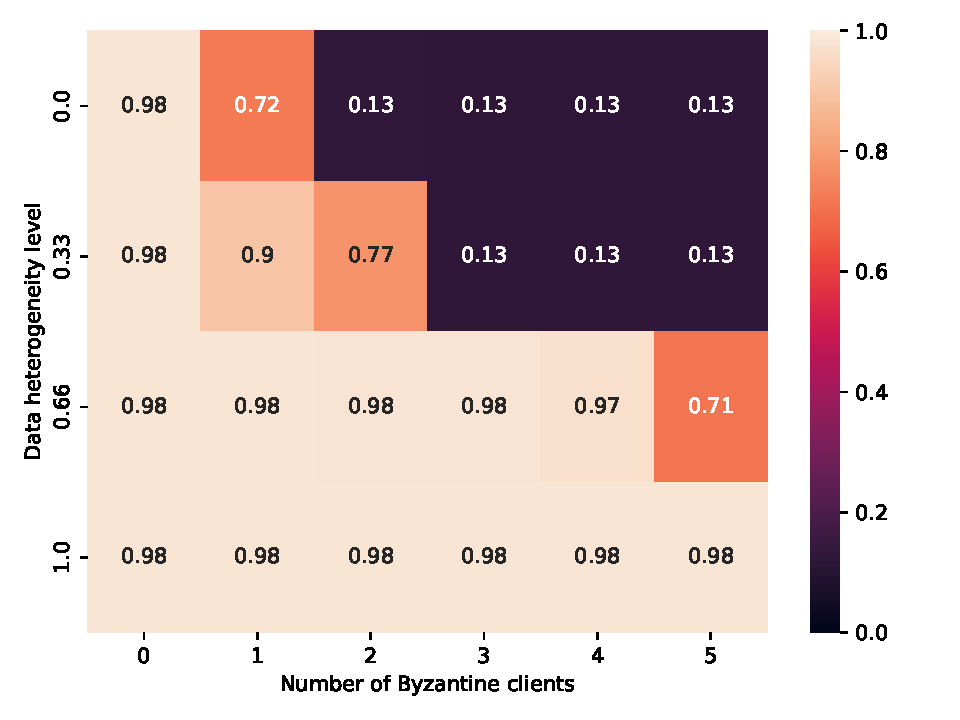
\includegraphics[width=\textwidth]{heatmap_alpha_3_0.pdf}
        \caption{$\alpha = 3.0$}
        \label{fig:alpha_3_0}
    \end{subfigure}
    
    \caption{Aggregated Test Accuracy Heatmaps across different surrogate gradient $\alpha$ values for SNN ($f \le 3$).}
    \label{fig:atan_alpha_heatmaps}
\end{figure}

\newpage

\section{Quantitative Performance Summary}
Table~\ref{tab:summary} compares the overall performance metrics for each $\alpha$ parameter value. The metrics include the average accuracy across all 16 cells in the grid, the worst-case accuracy, and the accuracy under the most challenging experimental setup ($\gamma=0.0$, $f=3$).

\begin{table}[htbp]
    \centering
    \caption{Performance Summary for Different Surrogate Gradient scaling values ($\alpha$).}
    \label{tab:summary}
    \begin{tabular}{lccc}
        \toprule
        \textbf{Surrogate Scaling ($\alpha$)} & \textbf{Average Accuracy} & \textbf{Worst-case Accuracy} & \textbf{Accuracy ($\gamma=0.0, f=3$)} \\
        \midrule
        $\alpha = 1.0$ & 87.52\% & 14.22\% & 14.22\% \\
        $\alpha = 1.25$ & 83.27\% & 13.42\% & 13.42\% \\
        $\alpha = 1.5$ & 82.91\% & 12.63\% & 12.63\% \\
        $\alpha = 2.0$ & 80.58\% & 12.63\% & 12.63\% \\
        $\alpha = 3.0$ & 78.73\% & 12.63\% & 12.63\% \\
        \bottomrule
    \end{tabular}
\end{table}

\section{Detailed Grid Tables for each $\alpha$}
This section lists the exact aggregated test accuracies for each data heterogeneity level ($\gamma$) and number of Byzantine clients ($f$).

\subsection{Surrogate scaling $\alpha = 1.0$}
\begin{table}[htbp]
    \centering
    \begin{tabular}{ccccc}
        \toprule
        & \textbf{f = 0} & \textbf{f = 1} & \textbf{f = 2} & \textbf{f = 3} \\
        \midrule
        $\gamma = 1.0$ & 96.43\% & 96.42\% & 96.48\% & 96.52\% \\
        $\gamma = 0.66$ & 96.43\% & 96.90\% & 96.98\% & 96.75\% \\
        $\gamma = 0.33$ & 96.46\% & 96.45\% & 95.44\% & 90.66\% \\
        $\gamma = 0.0$ & 96.41\% & 84.02\% & 53.80\% & 14.22\% \\
        \bottomrule
    \end{tabular}
\end{table}
\subsection{Surrogate scaling $\alpha = 1.25$}
\begin{table}[htbp]
    \centering
    \begin{tabular}{ccccc}
        \toprule
        & \textbf{f = 0} & \textbf{f = 1} & \textbf{f = 2} & \textbf{f = 3} \\
        \midrule
        $\gamma = 1.0$ & 97.01\% & 97.02\% & 97.09\% & 97.11\% \\
        $\gamma = 0.66$ & 97.10\% & 97.43\% & 97.37\% & 97.17\% \\
        $\gamma = 0.33$ & 97.04\% & 96.98\% & 95.77\% & 51.45\% \\
        $\gamma = 0.0$ & 97.04\% & 79.69\% & 23.57\% & 13.42\% \\
        \bottomrule
    \end{tabular}
\end{table}
\subsection{Surrogate scaling $\alpha = 1.5$}
\begin{table}[htbp]
    \centering
    \begin{tabular}{ccccc}
        \toprule
        & \textbf{f = 0} & \textbf{f = 1} & \textbf{f = 2} & \textbf{f = 3} \\
        \midrule
        $\gamma = 1.0$ & 97.36\% & 97.38\% & 97.42\% & 97.47\% \\
        $\gamma = 0.66$ & 97.37\% & 97.74\% & 97.45\% & 97.25\% \\
        $\gamma = 0.33$ & 97.31\% & 97.05\% & 95.82\% & 51.96\% \\
        $\gamma = 0.0$ & 97.39\% & 72.43\% & 22.55\% & 12.63\% \\
        \bottomrule
    \end{tabular}
\end{table}
\subsection{Surrogate scaling $\alpha = 2.0$}
\begin{table}[htbp]
    \centering
    \begin{tabular}{ccccc}
        \toprule
        & \textbf{f = 0} & \textbf{f = 1} & \textbf{f = 2} & \textbf{f = 3} \\
        \midrule
        $\gamma = 1.0$ & 97.82\% & 97.83\% & 97.88\% & 97.90\% \\
        $\gamma = 0.66$ & 97.85\% & 97.96\% & 97.86\% & 97.48\% \\
        $\gamma = 0.33$ & 97.81\% & 96.83\% & 95.80\% & 16.78\% \\
        $\gamma = 0.0$ & 97.79\% & 69.68\% & 19.39\% & 12.63\% \\
        \bottomrule
    \end{tabular}
\end{table}
\subsection{Surrogate scaling $\alpha = 3.0$}
\begin{table}[htbp]
    \centering
    \begin{tabular}{ccccc}
        \toprule
        & \textbf{f = 0} & \textbf{f = 1} & \textbf{f = 2} & \textbf{f = 3} \\
        \midrule
        $\gamma = 1.0$ & 98.19\% & 98.27\% & 98.24\% & 98.21\% \\
        $\gamma = 0.66$ & 98.23\% & 98.28\% & 98.02\% & 97.94\% \\
        $\gamma = 0.33$ & 98.17\% & 90.11\% & 77.40\% & 12.63\% \\
        $\gamma = 0.0$ & 98.11\% & 72.11\% & 13.18\% & 12.63\% \\
        \bottomrule
    \end{tabular}
\end{table}

\section{Key Interpretations}
Based on the sweep results:
\begin{itemize}
    \item \textbf{Optimal $\alpha$ Value}: Tuning the surrogate gradient scaling factor $\alpha$ has a significant impact on learning under non-IID conditions and Byzantine attacks. Larger $\alpha$ values tend to sharpen the gradient approximation, while smaller values smooth it.
    \item \textbf{Non-IID Stability}: The worst-case accuracy drops are mostly concentrated in the $\gamma = 0.0$ and $f = 3$ regime. Comparing this cell across different $\alpha$ values allows us to identify the most robust configurations.
\end{itemize}

\end{document}
